\section{Modelos de lenguaje}

Un <<modelo de lenguaje>> es un modelo estadístico que asigna una probabilidad a una secuencia de palabras dada como entrada. Esencialmente, es una función matemática diseñada para simular la forma en que se escribe en lenguaje natural. Una analogía común para entender el funcionamiento de un modelo de lenguaje es la función predictiva de un teclado. Mientras escribimos en nuestro dispositivo móvil, el teclado nos sugiere palabras que probablemente seguirán a las ingresadas. Esta capacidad de predicción es el fundamento de los modelos de lenguaje, incluyendo chatbots avanzados.

Desde una perspectiva técnica, un modelo de lenguaje devuelve como salida la distribución de probabilidad del siguiente \textit{token}, dada una secuencia de \textit{tokens} como entrada \citep{GenerationLLMs}. Un \textit{token} es la unidad mínima de información que el modelo procesa y, generalmente, equivale a una palabra\footnote{Aunque un token suele ser una palabra, también puede ser un signo de puntuación, número o cualquier otra unidad mínima de información.}. La Figura \ref{fig:llm_generation} ilustra un modelo de lenguaje que recibe una secuencia de palabras y devuelve la distribución de probabilidad del siguiente \textit{token} después de haber sido entrenado con textos en inglés.

\begin{figure}[H]
    \caption[Inferencia de \textit{token} de un LLM]{Inferencia de \textit{token} de un LLM}
    \centering
    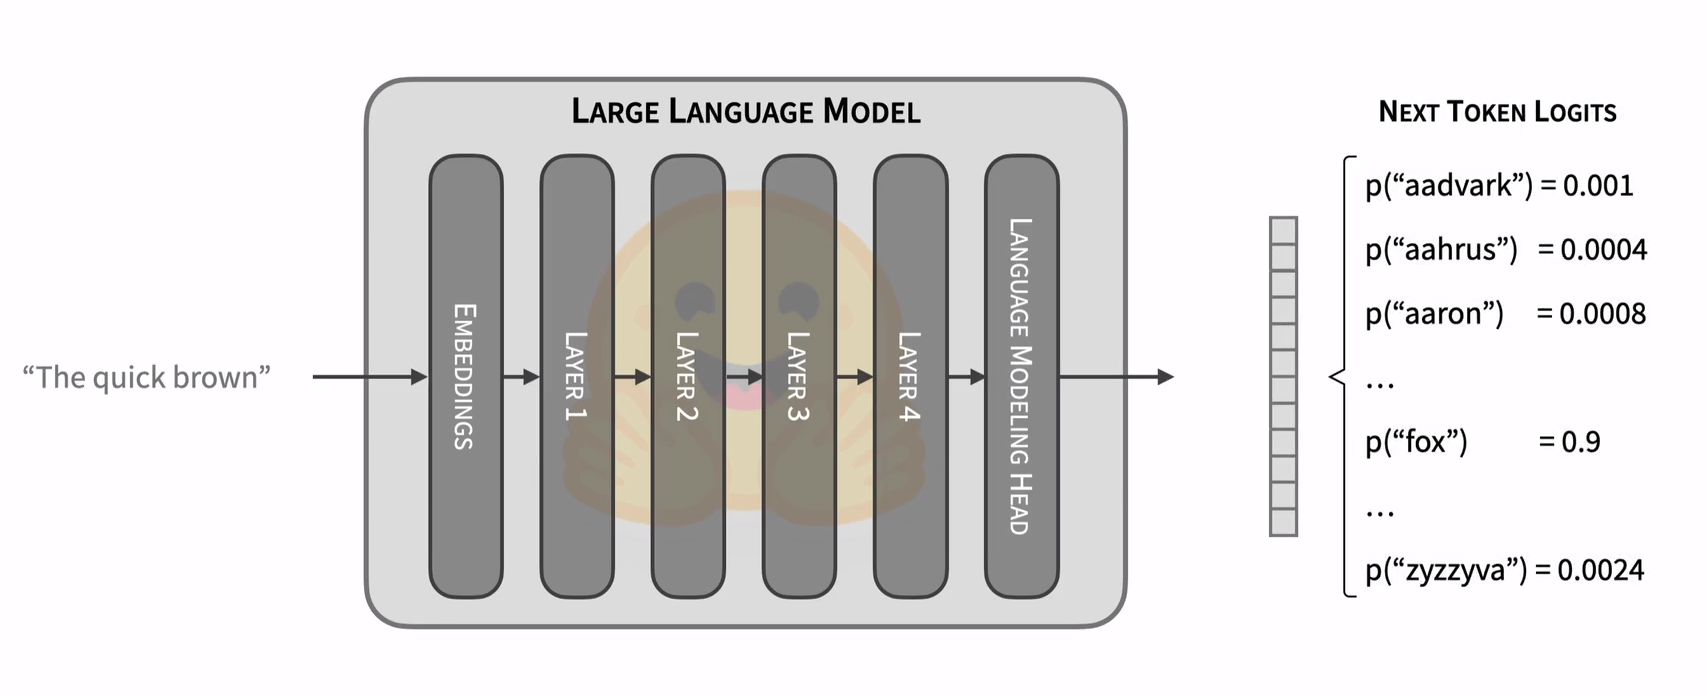
\includegraphics[width=0.9\textwidth]{./figuras/LLM_predice_token.png}
    \source{\cite{GenerationLLMs}}
    \label{fig:llm_generation}
\end{figure}

Los modelos de lenguaje no se asocian exclusivamente a una arquitectura de \gls{ml}. Pueden implementarse mediante diferentes tipos de redes neuronales, como las redes neuronales recurrentes o convolucionales. No obstante, el hito que ha propulsado avances significativos en \gls{ml} ha sido la arquitectura \textit{Transformer} \citep{vaswaniAttentionAllYou2017}, de la que se ha hablado más arriba.

\subsection{Grandes modelos de lenguaje}

Un \gls{llm} posee un número de parámetros del orden del billón, lo cual es considerado <<grande>> o \textit{large} desde el punto de vista computacional. El primer \gls{llm} fue \textit{GPT-2}, creado y entrenado por OpenAI en 2019 \citep{radfordLanguageModelsAre2019a}. \textit{GPT-2} se entrenó con 40 GB de texto de Internet y alcanzó 1.5 billones de parámetros. Su capacidad para predecir la siguiente palabra en una secuencia sorprendió a la comunidad científica debido a la calidad de los textos generados. Sin embargo, OpenAI publicó una versión reducida de 117 millones de parámetros debido a preocupaciones sobre su eventual uso irresponsable. La Figura \ref{fig:gpt2_text_generation} muestra ejemplos de textos generados por este modelo.

\begin{figure}[H]
    \caption{Generación de textos por \textit{GPT-2}}
    \centering
    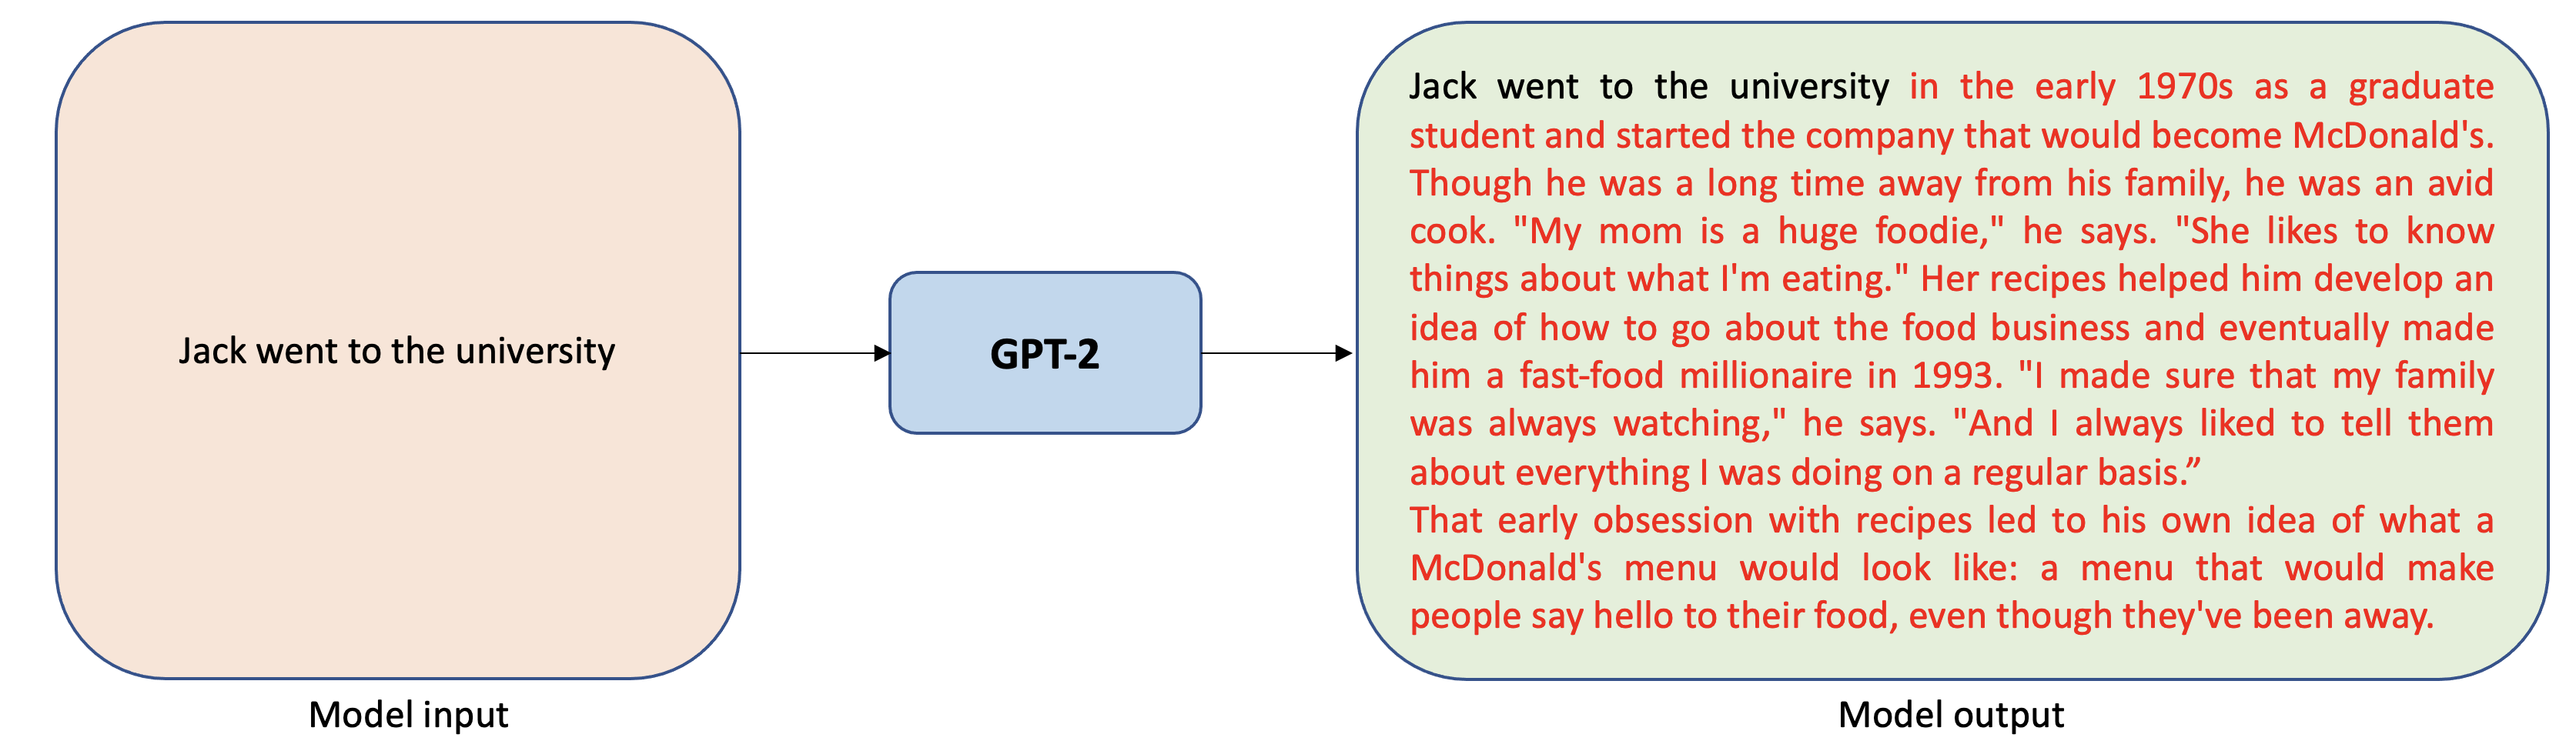
\includegraphics[width=0.9\textwidth]{./figuras/GPT2_text_generation.png}
    \source{\cite{RunTextGeneration2022}}
    \label{fig:gpt2_text_generation}
\end{figure}

Los \gls{llm} emplean la arquitectura \textit{Transformer} o derivados. Se entrenan con grandes cantidades de texto sin etiquetar, como libros, artículos de periódicos, páginas web, etc., realizándose este proceso en paralelo, lo que requiere una gran capacidad computacional. Sin embargo, una vez entrenados, estos modelos pueden ser utilizados para tareas de generación de texto, traducción automática, resumen de textos, etc. con una capacidad predictiva sorprendente. La Figura \ref{fig:llm_sizes} muestra una comparativa de los tamaños de los \gls{llm} más conocidos.

\begin{figure}[H]
    \caption{Gráfico comparativo de tamaños de LLM}
    \centering
    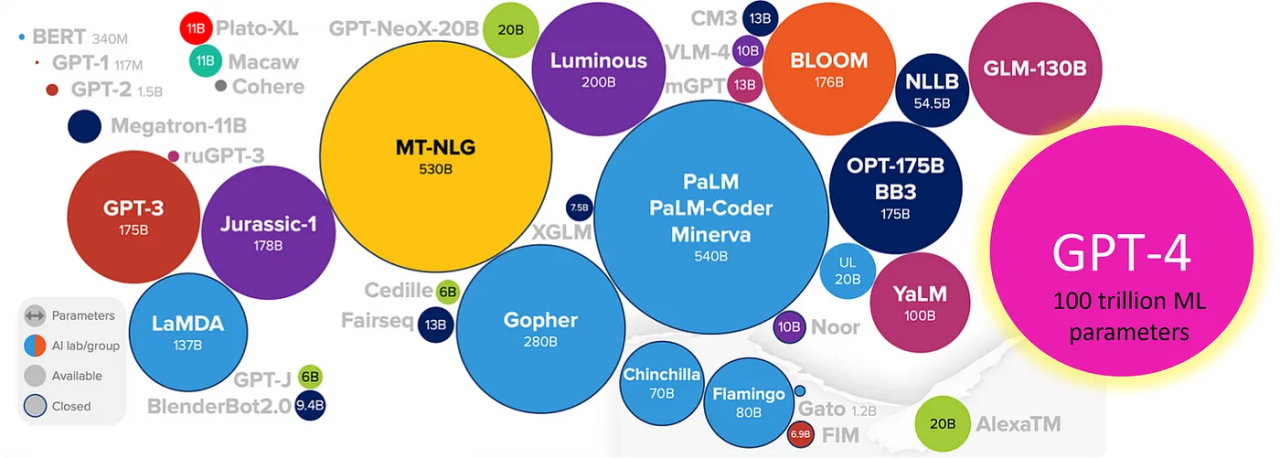
\includegraphics[width=0.9\textwidth]{./figuras/LLMs_sizes.png}
    \source{\cite{ChallengesAssociatedBuilding}}
    \label{fig:llm_sizes}
\end{figure}

\subsection{Modelos preentrenados}
\subsection{Ajuste fino de los modelos}
Bibliografía: \cite{chamandFinetuneYourClassifier2022}

\subsection{Hiperparámetros fijos del modelo}
Aquí hablaré de los hiperparámetros que definen la arquitectura del modelo que no se pueden modificar, como el número de capas, el número de cabezas de atención, etc., y que son fijos en el modelo. Especial atención se pondrá en el número de parámetros del modelo, que es el que determina el tamaño del modelo y su capacidad de generar textos, así como en la ventana de contexto, que es el número de \textit{tokens} que el modelo tiene en cuenta para generar el siguiente token.

Precisamente el número de parámetros y la ventana de contexto son los hiperparámetros más importantes y críticos en términos computacionales y de efectividad. Cuanto más grande sea el modelo, más parámetros tendrá y más capacidad de generar textos tendrá. Sin embargo, también será más lento en la inferencia. Por otro lado, cuanto mayor sea la ventana de contexto, más \textit{tokens} tendrá en cuenta el modelo para generar el siguiente token, y más coherentes serán los textos generados. Sin embargo, también será más lento en la inferencia.

Consideraciones interesantes sobre parámetros y ventana de contexto en \cite{gonzaloAsomandonosVentanaContextual2023}

\subsection{Hiperparámetros controlables por el usuario}
\label{sec:hiperparametros_controlables}
Hablar de la temperatura, top\_p, top\_k, ventana de contexto, número de \textit{tokens}, etc. 

Se habla de la temperatura y su impacto en la generación de textos en \cite{holtzmanCuriousCaseNeural2020} y \cite{chamandFinetuneYourClassifier2022}

\cite{holtzmanCuriousCaseNeural2020} habla de la importancia de top\_p, en lo que denomina \textit{top\_k nucleus sampling}. Aunque es antiguo el paper, echar un ojo porque aclara bastante los conceptos.

Seguimos las explicaciones de \cite{rothmanTransformersNaturalLanguage2021}

Existen estudios centrados en la optimización de los hiperparámetros (los ya citados más arriba y \cite{wangCostEffectiveHyperparameterOptimization2023} y \cite{wangHyperparameterOptimizationAlgorithm2022})

